\documentclass[11pt,a4paper]{article}

\usepackage{geometry}
 \geometry{
 a4paper,
 total={150mm,237mm},
 left=30mm,
 top=30mm,
 }

% cf. http://tex.stackexchange.com/questions/50182/subtitle-with-the-maketitle-page
\usepackage{titling}
\newcommand{\subtitle}[1]{%
  \posttitle{%
    \par\end{center}
    \begin{center}\large\textbf{#1}\end{center}
    \vskip0.5em}%
}

\usepackage{color}
\usepackage{graphicx}
\usepackage{subcaption}

\usepackage[utf8]{inputenc}
\usepackage[lf]{venturis} %% lf option gives lining figures as default; 
\usepackage[T1]{fontenc}
\usepackage{csquotes}
\usepackage[UKenglish,german]{babel}

\usepackage{fancyvrb}

\widowpenalty10000  % http://tex.stackexchange.com/questions/4152/how-do-i-prevent-widow-orphan-lines
\clubpenalty10000

\title{The SysSon Platform}
\subtitle{Technical Report TR-2016-09-1\\Institute of Electronic Music and Acoustics, Graz\\(Status: completed)}
\author{Hanns Holger Rutz}
% \date{09-Feb-2016}
\date{September 2016}

% cf. https://tex.stackexchange.com/questions/94126/change-font-to-only-section-and-subsection-of-my-document
%\usepackage{titlesec}
%\titleformat{\chapter}[display]
%  {\fontfamily{pag}\selectfont\huge\bfseries}
%  {\chaptertitlename\ \thechapter}
%  {20pt}
%  {\Huge}
%\titleformat{\section}
%  {\fontfamily{pag}\selectfont\bfseries\Large}
%  {\thesection}
%  {1em}
%  {}
%\titleformat{\subsection}
%  {\fontfamily{pag}\selectfont\bfseries\Large}
%  {\thesection}
%  {1em}
%  {}

\usepackage[backend=biber,authordate]{biblatex-chicago} % citereset=chapter
%\usepackage[backend=biber,natbib,isbn=false,useprefix=true,sorting=ydnt]{biblatex-chicago} % citereset=chapter
\addbibresource{all.bib} % add a bib-reference file
\addbibresource{rutz.bib} % add a bib-reference file

% warning: https://tex.stackexchange.com/questions/313477/
% \usepackage{csquotes}

\usepackage{tabularx}
% cf. https://tex.stackexchange.com/questions/84400/table-layout-with-tabularx-column-widths-502525
\newcolumntype{s}{>{\hsize=1cm}X}

% says you should load after babel and fontspec
\usepackage[shrink=10, babel=true]{microtype}	% http://tex.stackexchange.com/questions/141852/latex-allows-line-break-between-concluding-em-dash-and-comma-before-a-new-sub-cl/141854#141854

% has to come first for full scale TeX voodoo bullcrap
\usepackage{hyperref}
% get rid of the horrible coloured boxes around links
\hypersetup{
    colorlinks,%
    citecolor=black,%
    filecolor=black,%
    linkcolor=black,%
    urlcolor=black
}
% has to come after frickin hyperref
\VerbatimFootnotes

\newcommand{\todo}[1]{\colorbox{yellow}{\textsc{todo}: #1}}

\newcommand{\quot}[1]{\guillemotleft {#1}\guillemotright}

\newcommand{\worktitle}[1]{\textit{#1}}

\newcommand{\workentry}[2]{\vspace{7.5pt}\noindent\textbf{#1} (#2)}
\newcommand{\workentrySel}[2]{\vspace{7.5pt}\noindent\textbf{#1}$*$ (#2)}

\newcommand{\figref}[1]{Fig.~\ref{#1}}

\newcommand{\software}[1]{\textit{#1}}

\newcommand{\sysson}[0]{SysSon}
\newcommand{\syssonVersion}[0]{1.8.0}
\newcommand{\syssonVersionS}[0]{1.8.0-SNAPSHOT}

\newcommand{\artefacts}[0]{\textsc{Artefacts:}}
\newcommand{\assessment}[0]{\textsc{Assessment:}}

\begin{document}
% \begin{titlepage}
\maketitle
\selectlanguage{UKenglish}
\thispagestyle{empty}
\newpage
\section{Implementation of If-Branch}

A small DSL is provided that allows the definition of conditional branches using a syntax relatively close to standard Scala `if/else` blocks. The following shows the example scenario to test the implementation:
%
\begin{verbatim}
SynthGraph {
  val amp : GE = "amp" .kr(0.2)
  val freq: GE = "freq".kr

  val res0: GE = 
    If (freq > 1000) Then {
      SinOsc.ar(freq)
    } ElseIf (freq > 100) Then {
      Dust.ar(freq)
    } Else {
      WhiteNoise.ar
    }

  Out.ar(0, Pan2.ar(res0 * amp))
}
\end{verbatim}
%
We first have a \textbf{``monolithic''} implementation that rewrites this graph into one single UGen graph where all branches are always computed but the resulting signal \Verb!res0! only contains the signal of the ``active'' branch. The UGen graph is shown in \figref{fig:ugen-mono}. Basically the branch signals are multiplied by the logical branch condition (a graph element that is forced to be zero or one) and then summed up.

\begin{figure}
\centering
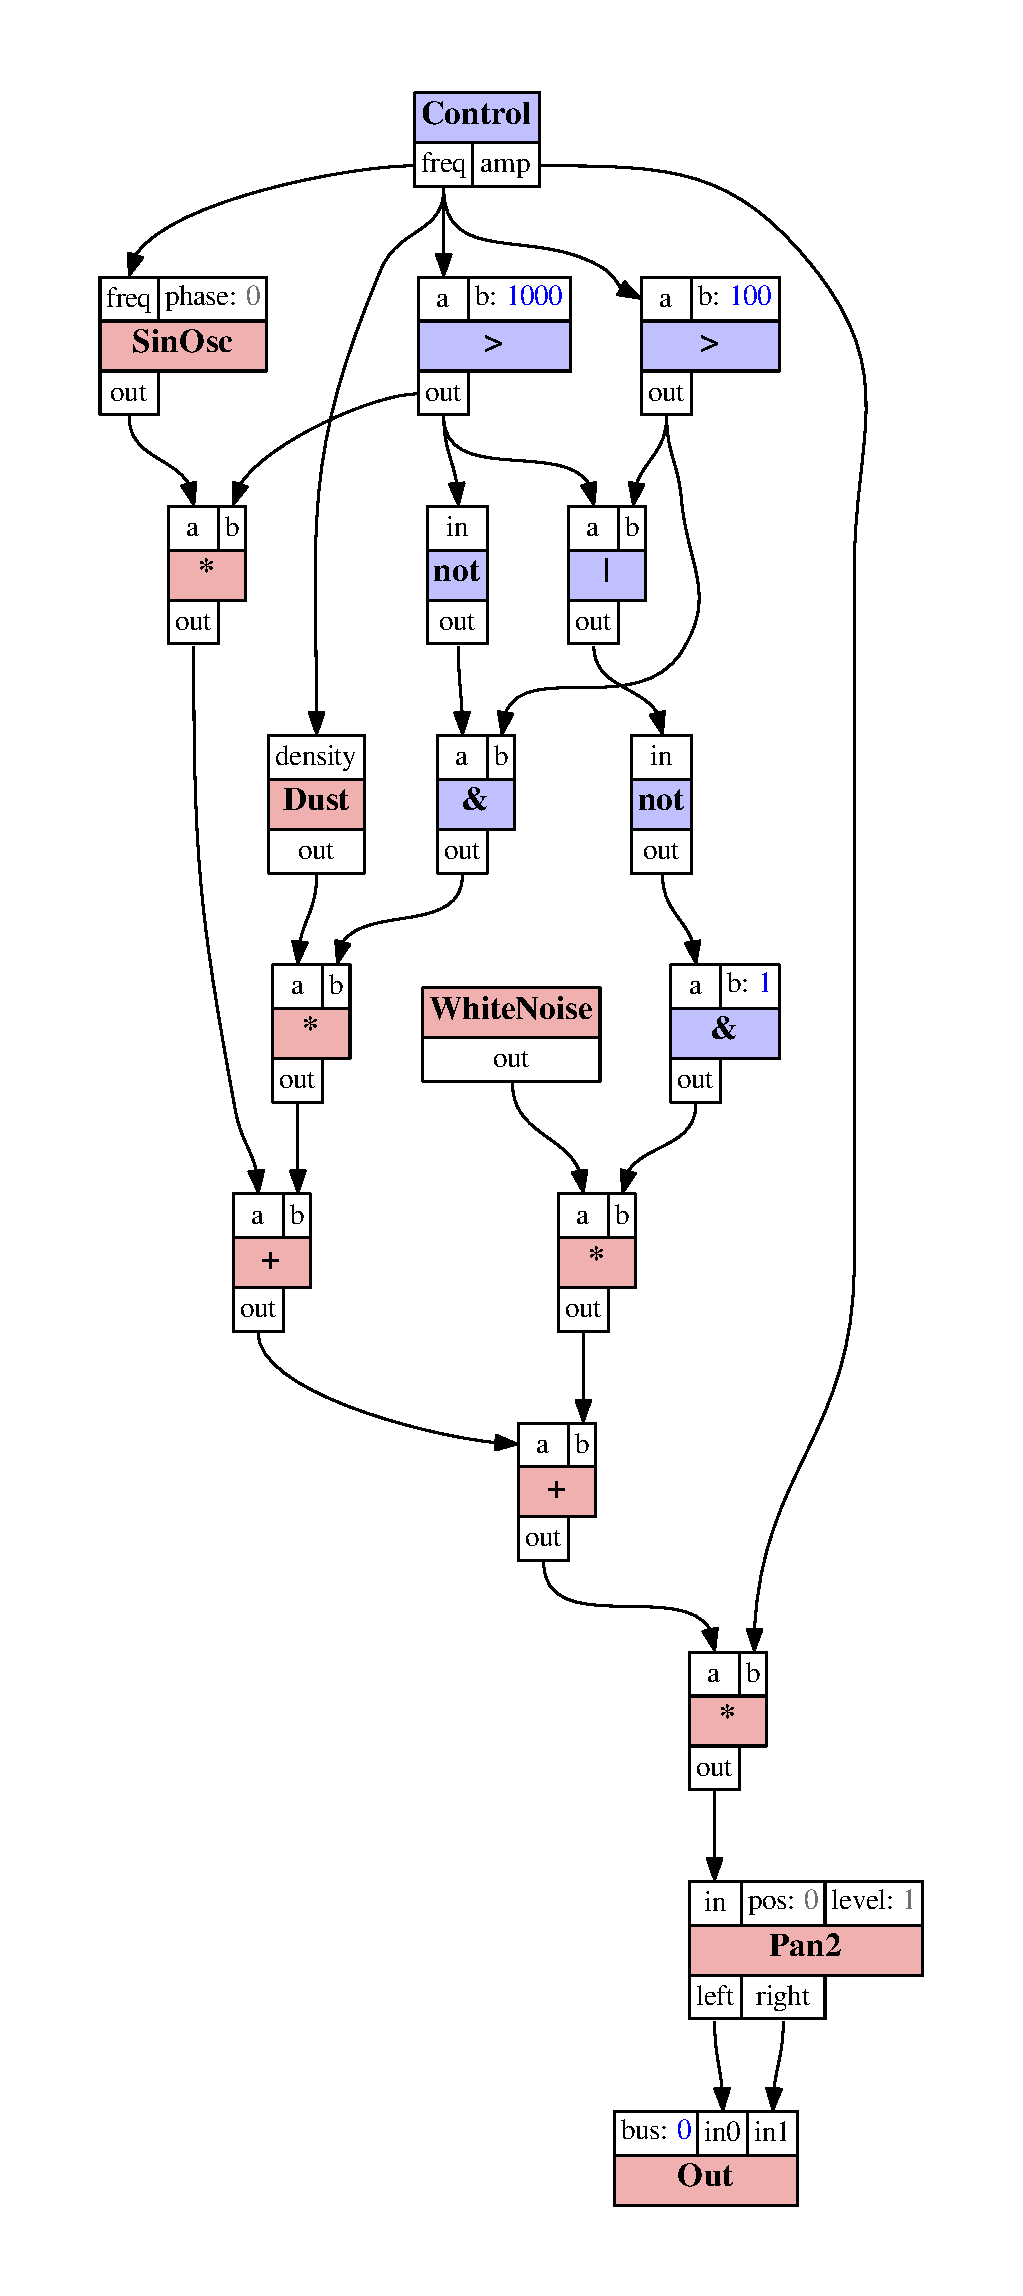
\includegraphics[scale=0.5]{figures/ugen-if-mono.pdf}
\caption{``Monolithically'' expanded synth graph.}
\label{fig:ugen-mono}
\end{figure}

The second implementation then actually performs the \textbf{modular} decomposition into a set of related UGen graphs. Each conditional branch becomes a child UGen graph that will be run in its own \Verb!Synth! instance. Using a \Verb!Group! we can share the same control signals among them. For example, a control is specified for the ``return bus'' to which all branches are adding up their output. The main graph uses \Verb!Pause! UGens to start and stop the branches, receiving additional controls for the node-identifiers of the children. If a branch refers to elements from the outer context, auxiliary buses are established. In the example, the \Verb!freq! control signal is used by the main body (because it forms part of the branch-conditions that are tested here) and inside two of the three branches. Therefore, the main graph routes this signal to an auxiliary bus using an \Verb!Out! UGen, and that signal is then read by the respective child branches using an \Verb!In! UGen.

\begin{figure}
\centering
\begin{subfigure}[b]{0.6\textwidth}%
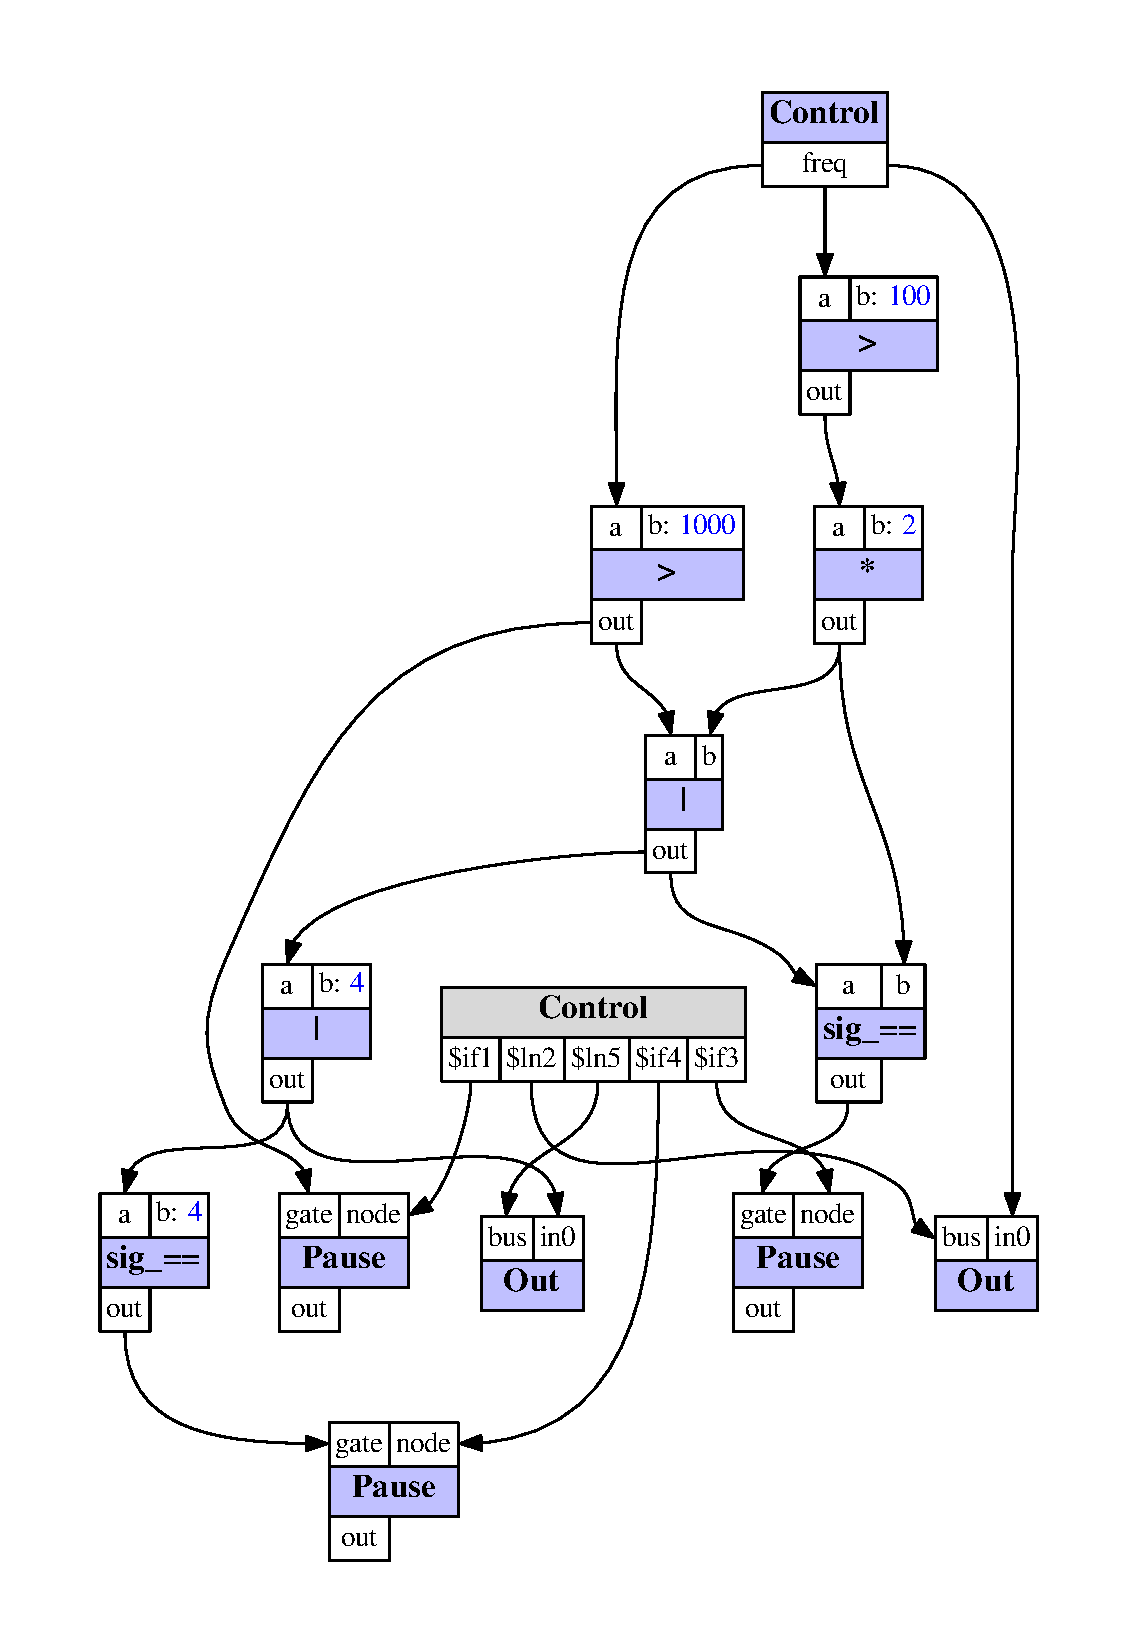
\includegraphics[scale=0.5]{figures/ugen-if-mod-top.pdf}
\caption{Top level}\label{fig:ugen-mod-top}
\end{subfigure}
\begin{subfigure}[b]{0.3\textwidth}%
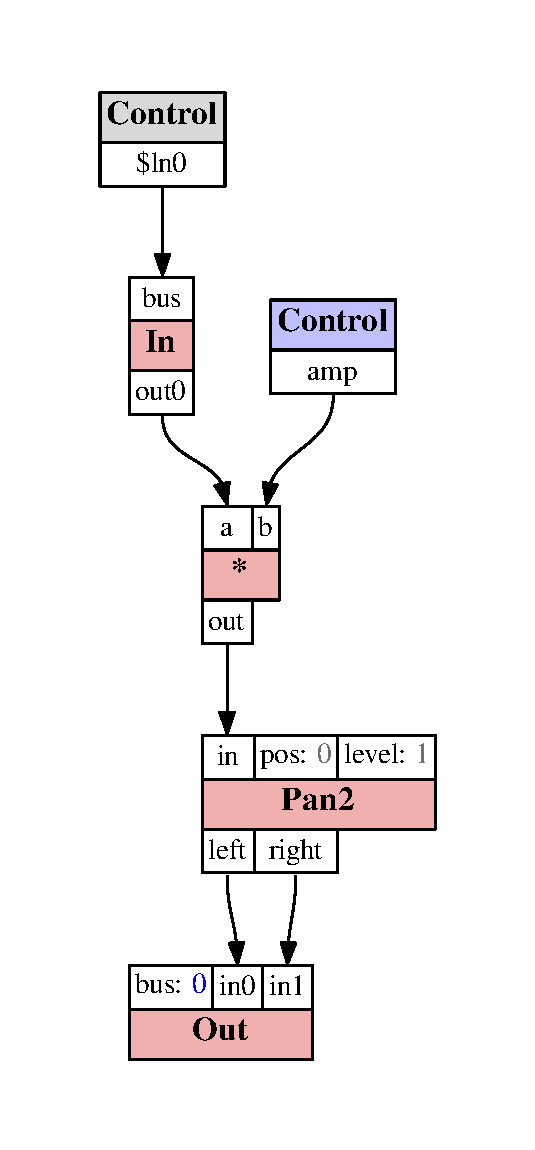
\includegraphics[scale=0.5]{figures/ugen-if-mod-child_4.pdf}
\caption{Child 4 (top-level sink)}\label{fig:ugen-mod-c4}
\end{subfigure}
\begin{subfigure}[b]{0.3\textwidth}%
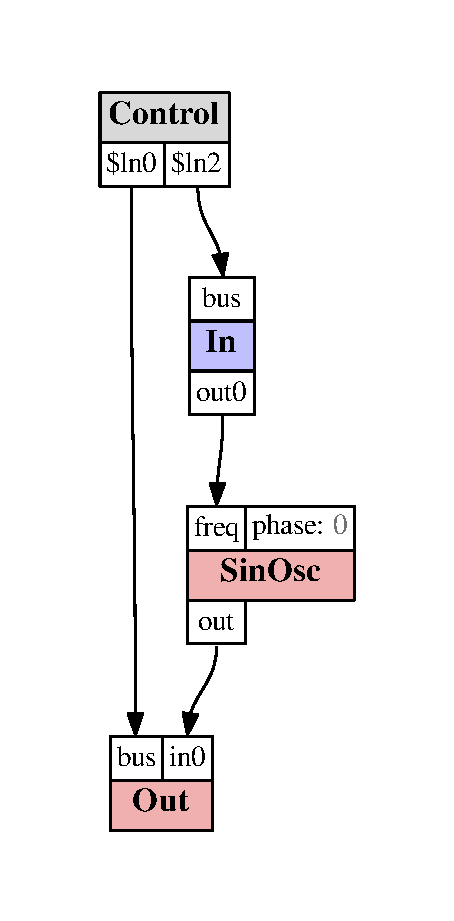
\includegraphics[scale=0.5]{figures/ugen-if-mod-child_1.pdf}
\caption{Child 1 (if-branch)}\label{fig:ugen-mod-c1}
\end{subfigure}
\begin{subfigure}[b]{0.3\textwidth}%
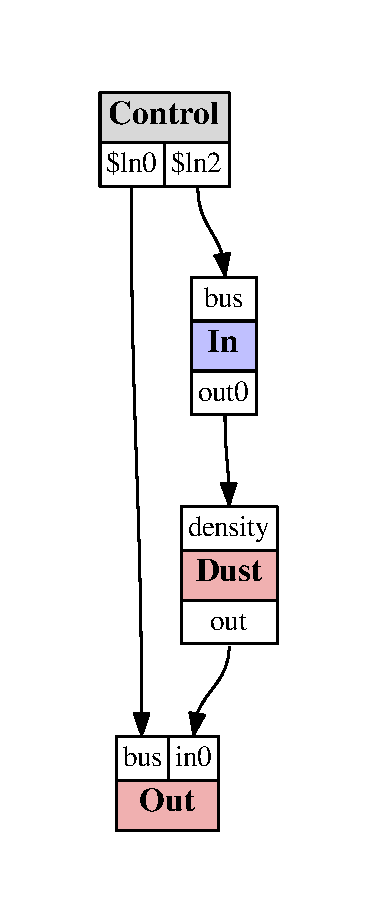
\includegraphics[scale=0.5]{figures/ugen-if-mod-child_2.pdf}
\caption{Child 2 (else-if-branch)}\label{fig:ugen-mod-c2}
\end{subfigure}
\begin{subfigure}[b]{0.3\textwidth}%
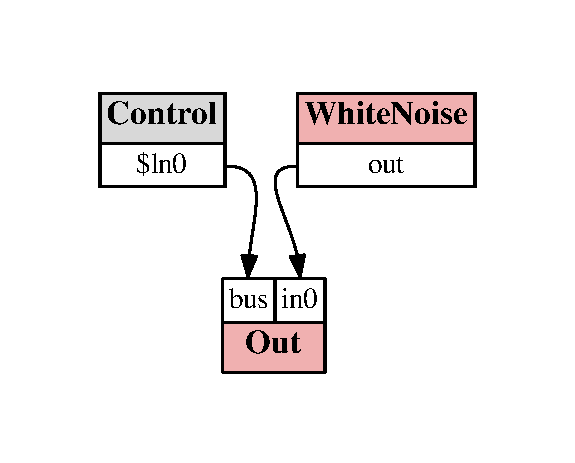
\includegraphics[scale=0.5]{figures/ugen-if-mod-child_3.pdf}
\caption{Child 3 (else-branch)}\label{fig:ugen-mod-c3}
\end{subfigure}
\caption{Modular expanded synth graph.}
\label{fig:ugen-modular}
\end{figure}

Several possibilities of handling the ``return signal'' have been evaluated, and the implementation settled on a simple and straight forward construction, whereby the property of the acyclicity of the directed graph implies that dependants on the branch signals can only occur after them in the sequence of graph elements registered with the \Verb!SynthGraph!. We thus initiate a new child branch after having visited any if-branch whose return type is \Verb!GE!. In other words, \Verb!Out.ar(0, Pan2.ar(res0 * amp))! will be encapsulated in another (forth) child branch.

\newpage
\subsection{ThisBranch}

A branch may want to react to the fact that is selected. For example, an envelope might need to be restart, some UGen state might need to be reset. To facilitate this, a new graph element \Verb!ThisBranch! is introduced:
%
\begin{verbatim}
val act = "active".kr
val res: GE = If (act) Then {
  val tr = ThisBranch()
  val freq = Sweep.kr(tr, 0.5).min(1.0).linexp(0, 1, 200, 2000)
  SinOsc.ar(freq) * 0.2
} Else {
  val tr  = ThisBranch()
  val amp = Sweep.kr(tr, 0.5).min(1.0).linexp(0, 1, -40.dbamp, 0.dbamp)
  WhiteNoise.ar(amp)
}
Out.ar(0, Pan2.ar(res))
\end{verbatim}

\subsection{IfLag}

We also want to be able to specify a fade-out time in seconds. We distinguish between fade-out phase and normal state. During fade-out phase, changes in conditionals have no effect. Once the fade-out is complete, the conditionals take effect again. This means that if the branch changes fast from one to two back to one, we might not actually pause the first branch and resume the second one, but simply fade out the first and then fade it back in (retrigger \Verb!ThisBranch!).

The implementation changes from trigger to gate signal for \Verb!ThisBranch!. This is achieved by adding a release period of the given duration when the branch index changes. In this period, the old index is still held, but the gate signal goes low. Any changes in the index during the release are blocked out. Once the release has completed, the current index is let throw and causes a new branch to be resumed with a high gate signal.

Here is an example:
%
\begin{verbatim}
SynthGraph {
  val tr    = Impulse.kr(ControlRate.ir / 15)
  val ff    = ToggleFF.kr(tr)
  val dur   = ControlDur.ir * 5
  val res   = IfLag (ff, dur) Then {
    val gate  = ThisBranch()
    val env   = Env.asr(attack = dur, release = dur, curve = Curve.lin)
    val eg    = EnvGen.ar(env, gate)
    Seq(eg, DC.ar(0)): GE
  } Else {
    val gate  = ThisBranch()
    val env   = Env.asr(attack = dur, release = dur, curve = Curve.lin)
    val eg    = EnvGen.ar(env, gate)
    Seq(DC.ar(0), eg): GE
  }
  Out.ar(0, res)
}
\end{verbatim}
%
The corresponding phase diagram is shown in \figref{fig:iflag-gate}. Because there is no release phase in the very beginning, the period where the first signal has a high gate is longer. Then one can see that the release of the previous branch does not overlap with the attach of the next branch. No two nodes are computed at the same time.

\begin{figure}
\centering
\begin{subfigure}[b]{1.0\textwidth}%
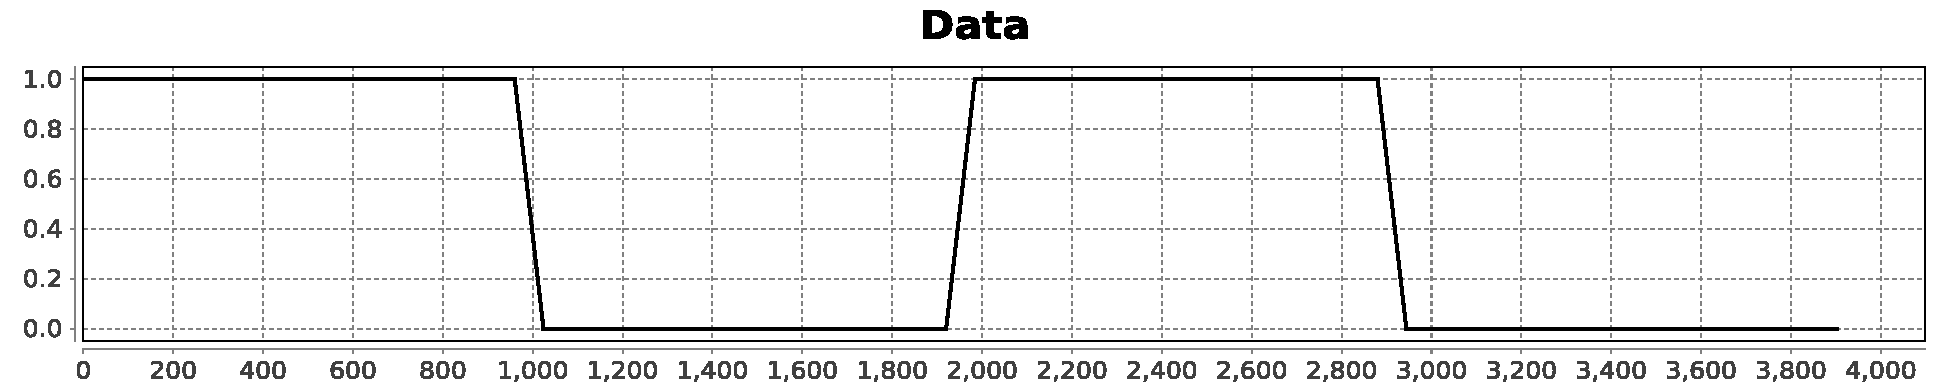
\includegraphics[width=\textwidth,trim=0 0 25mm 8mm,clip]{figures/iflag-cond-1.pdf}
\caption{The flip-flop signal used as condition for the first branch \\\phantom{(a) }(the linear slopes are an artifact resulting from converting a k-rate to an a-rate signal)}\label{fig:iflag-cond-1}
\end{subfigure}
\begin{subfigure}[b]{1.0\textwidth}%
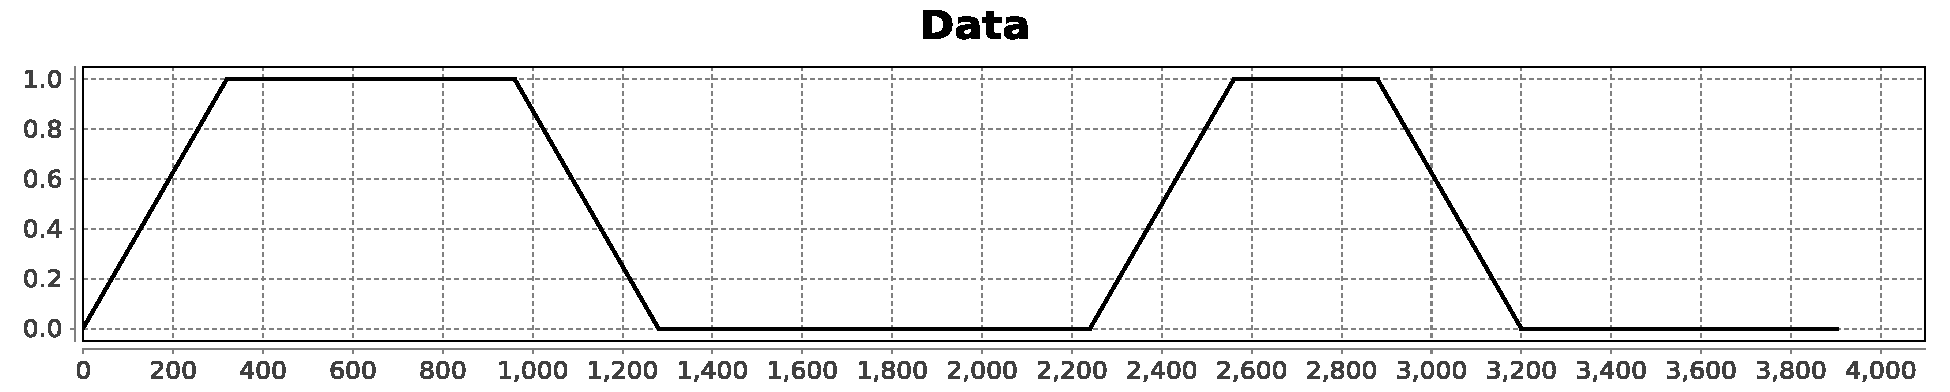
\includegraphics[width=\textwidth,trim=0 0 25mm 8mm,clip]{figures/iflag-gate-1.pdf}
\caption{Gate signal of the If-Then branch}\label{fig:iflag-gate-1}
\end{subfigure}
\begin{subfigure}[b]{1.0\textwidth}%
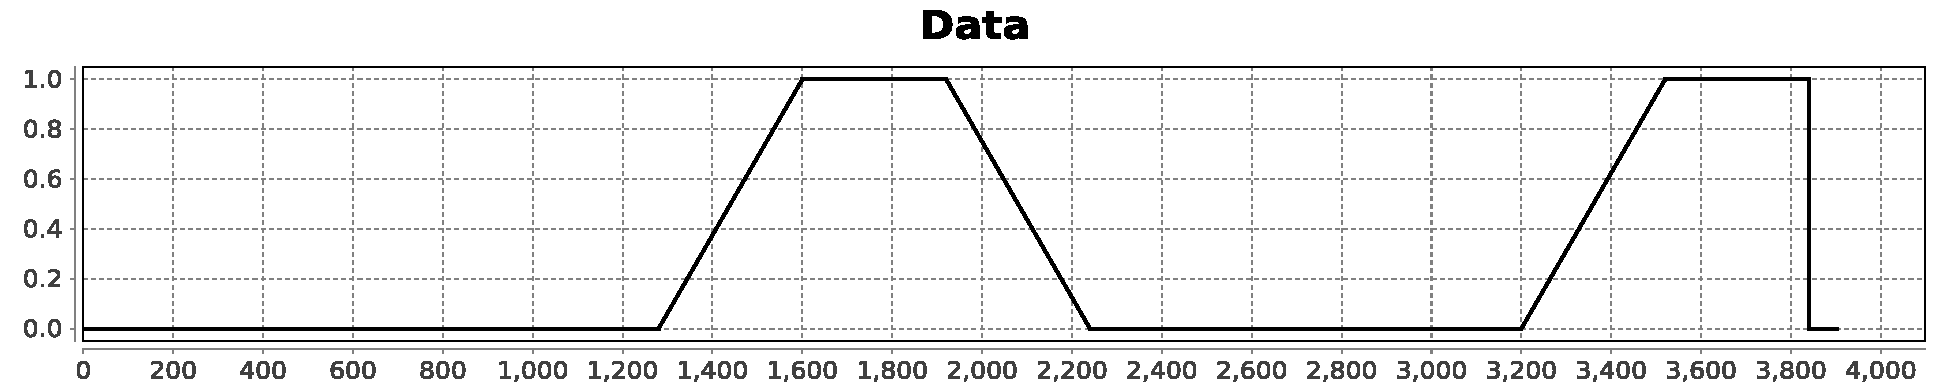
\includegraphics[width=\textwidth,trim=0 0 25mm 8mm,clip]{figures/iflag-gate-2.pdf}
\caption{Gate signal of the Else branch}\label{fig:iflag-gate-1}
\end{subfigure}
\caption{Phase diagram for an IfLag block with two branches}
\label{fig:iflag-gate}
\end{figure}

\section{Integration of If-elements with Sound\,Processes}

The UGen graph builder in \software{Sound\,Processes} was based on the basic building block in \software{ScalaCollider}, and operated in an ``incremental'' fashion: For each graph element expanded, it made a copy of the current state of the builder (controls, UGens expanded so far, etc.), then tried to expand the element. If in the course of this expansion a missing context property is detected, such as a missing attribute map entry, an exception is thrown, and the state is reset to the previous stable state.

Incorporating the \Verb!NestedUGenGraphBuilder! from the \software{ScalaCollider-If} library makes this even more complicated, because now state goes as deep as updating the child branches of an if-block. While it is not impossible to preserve this state, the bookkeeping will become very large, and therefore we must assess the value of the incremental build.

The original concept of the incremental build was that two graphs could co-dependent on each other, i.e. there might be a situation where two graphs could only be completely expanded, if each had partial knowledge about the other, usually in terms of the number of channels used for some particular output or input. So the vision was that for example the first graph could be half built, producing some knowledge that would then be needed by the other graph, and the second half of the first graph could only be completed once the other graph successfully provided some information.

But is this really a common scenario? From observing debugging sessions, it can be said that:
%
\begin{itemize}
\item incremental build is prone to bugs, because updating correctly as new information enters the system is difficult, and rolling back is also difficult.
\item often the element that requires the missing information is deep in the graph, which means that building the graph does not advance very far, so the advantage of having keeping already expanded elements becomes moot. It might be just as fast building the graph completely from scratch in the second and third attempt.
\end{itemize}
%
Therefore, if the incremental is dropped, we may get rid of a lot of complexity, and probably performance is not affected at all. The disadvantage is that large parts of the \Verb!AuralProcImpl! will have to be rewritten. On the other hand, we know that this class has bugs for many corner cases, and cleaning it up may benefit \software{SysSon} in the longer term.

\paragraph{Solution:} We dropped indeed the incremental graph build in favour of a more simple approach where the arrival of missing attribute entries leads to an entire rebuild of the graph.

\subsection{Release}

The implementation has been released as a separate library: \url{https://github.com/iem-projects/ScalaCollider-If}, and \software{Sound\,Processes} beginning from version 3.6.0 incorporates this into its own graph building. It is available in \software{SysSon} from version 1.9.0.

\subsection{Remaining Work}

\begin{itemize}
\item We want to foresee the possibility to match for i-rate conditions that can be resolved at graph expansion time, for example because the condition evaluates to a constant number. In that case, we can avoid creating sub-graphs for each branch but simply synthesise the branch that is always active. This exercise is not just a tweak for performance, but will be useful for evaluating constants coming from an \Verb!Obj!'s attribute map in \software{Sound\,Processes}.
\end{itemize}

% \printbibliography

\end{document}